%%%%%%%%%%%%%%%%%%%%%%%%%%%%%%%%%%%%%%%%%
% a0poster Portrait Poster
% LaTeX Template
% Version 1.0 (22/06/13)
%
% The a0poster class was created by:
% Gerlinde Kettl and Matthias Weiser (tex@kettl.de)
%
% This template has been downloaded from:
% http://www.LaTeXTemplates.com
%
% License:
% CC BY-NC-SA 3.0 (http://creativecommons.org/licenses/by-nc-sa/3.0/)
%
%%%%%%%%%%%%%%%%%%%%%%%%%%%%%%%%%%%%%%%%%

%----------------------------------------------------------------------------------------
%	PACKAGES AND OTHER DOCUMENT CONFIGURATIONS
%----------------------------------------------------------------------------------------

\documentclass[a0,portrait]{a0poster}

\usepackage{multicol} % This is so we can have multiple columns of text side-by-side
\columnsep=100pt % This is the amount of white space between the columns in the poster
\columnseprule=3pt % This is the thickness of the black line between the columns in the poster

\usepackage[svgnames]{xcolor} % Specify colors by their 'svgnames', for a full list of all colors available see here: http://www.latextemplates.com/svgnames-colors

%\usepackage{times} % Use the times font
\usepackage{palatino} % Uncomment to use the Palatino font

\usepackage{graphicx} % Required for including images
\graphicspath{{figures/}} % Location of the graphics files
\usepackage{booktabs} % Top and bottom rules for table
\usepackage[font=small,labelfont=bf]{caption} % Required for specifying captions to tables and figures
\usepackage{amsfonts, amsmath, amsthm, amssymb} % For math fonts, symbols and environments
\usepackage{wrapfig} % Allows wrapping text around tables and figures

\begin{document}

%----------------------------------------------------------------------------------------
%	POSTER HEADER
%----------------------------------------------------------------------------------------

% The header is divided into two boxes:
% The first is 75% wide and houses the title, subtitle, names, university/organization and contact information
% The second is 25% wide and houses a logo for your university/organization or a photo of you
% The widths of these boxes can be easily edited to accommodate your content as you see fit
\begin{minipage}[b]{0.75\linewidth}
  \veryHuge \color{NavyBlue} \textbf{\textsc{Does structure in neural \\[0.3cm] activity match anatomical structure?}} \color{Black}\\[1cm] % Title
  % \Huge\textit{An Exploration of Complexity}\\[2cm] % Subtitle
  \huge \textbf{Thomas Delaney, Dr. Cian O'Donnell}\\[0.3cm] % Author(s)
  \huge University of Bristol, Dept of Computer Science\\[0.1cm] % University/organization
  \large \texttt{bristolcnu.github.io} \\
  \Large \texttt{t.delaney@bristol.ac.uk} \\
\end{minipage}
%
\begin{minipage}[b]{0.24\linewidth}
  \centering
  
\includegraphics[width=0.9\linewidth]{bristol_university_logo.png} \vspace{0.3cm}\\
  
\includegraphics[width=0.9\linewidth]{epsrc_logo.png} \vspace{2.7cm}\\
\end{minipage}
%\vspace{0.5cm} % A bit of extra whitespace between the header and poster content

%----------------------------------------------------------------------------------------

\begin{multicols}{2} % This is how many columns your poster will be broken into, a portrait poster is generally split into 2 columns

%----------------------------------------------------------------------------------------
%	ABSTRACT
%----------------------------------------------------------------------------------------
%
% \color{Navy} % Navy color for the abstract
%
% \begin{abstract}
%
% Sed fringilla tempus hendrerit. Vestibulum ante ipsum primis in faucibus orci luctus et ultrices posuere cubilia Curae; Etiam ut elit sit amet metus lobortis consequat sit amet in libero. Lorem ipsum dolor sit amet, consectetur adipiscing elit. Phasellus vel sem magna. Nunc at convallis urna. isus ante. Pellentesque condimentum dui. Etiam sagittis purus non tellus tempor volutpat. Donec et dui non massa tristique adipiscing. Quisque vestibulum eros eu. Phasellus imperdiet, tortor vitae congue bibendum, felis enim sagittis lorem, et volutpat ante orci sagittis mi. Morbi rutrum laoreet semper. Morbi accumsan enim nec tortor consectetur non commodo nisi sollicitudin. Proin sollicitudin. Pellentesque eget orci eros. Fusce ultricies, tellus et pellentesque fringilla, ante massa luctus libero, quis tristique purus urna nec nibh.
%
% \end{abstract}

%----------------------------------------------------------------------------------------
%	INTRODUCTION
%----------------------------------------------------------------------------------------

%\color{SaddleBrown} % SaddleBrown color for the introduction

\section*{\color{NavyBlue}\textsc{Introduction}\color{Black}}

Information in the brain is carried in correlated network activity. Until recently, it has been difficult to record responses from multiple brain regions simultaneously. This meant that studies on network behaviour were restricted to studying only one region at a time. The development of `Neuropixels' probes have allowed extracellular voltage measurements to be collected from multiple brain regions simultaneously. In this project, we used data collected from five different brain regions to compare distributions of correlated activity within these regions, and between these regions.

We then used these measurements to create networks between the neurons in these five regions. We used a cutting edge community detection algorithm to find communities in these networks. We are currently in the process of comparing these communities to the anatomical distribution of their constituents.

%----------------------------------------------------------------------------------------
%	OBJECTIVES
%----------------------------------------------------------------------------------------

% \color{DarkSlateGray} % DarkSlateGray color for the rest of the content

\section*{\color{NavyBlue}\textsc{Main Objectives}\color{NavyBlue}}

\begin{enumerate}
  \item To compare the distributions of spike count correlations ($r_{SC}$) and mutual information ($I(X;Y)$) in different regions.
  \item To detect any communities in the networks created by these measurements, either within or between the anatomical regions.
  \item To compare the communities detected in the spike count correlation networks to those detected in the mutual information networks.
  \item To compare the network communities to their anatomical distribution.
\end{enumerate}

%----------------------------------------------------------------------------------------
%	DATA
%----------------------------------------------------------------------------------------

\section*{\color{NavyBlue}\textsc{Data}\color{NavyBlue}}

  Using two probes, spiking activity was simultaneously collected from over 800 neurons in an awake mouse brain for a period of 84 minutes. During this period, the mouse and was shown various visual stimuli. The 800 neurons were distributed across 5 different brain regions: \textbf{V1, hippocampus, thalamus, motor cortex}, and \textbf{striatum}.

\begin{center}\vspace{1cm}
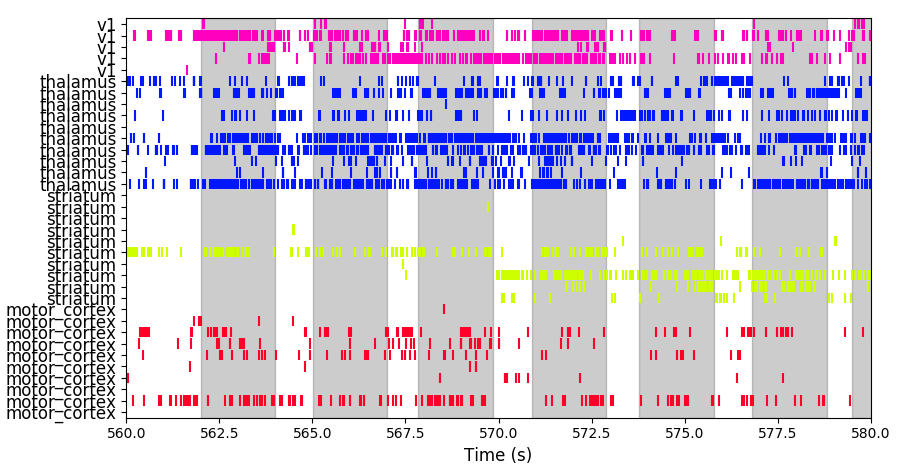
\includegraphics[width=0.8\linewidth]{raster_plot.png}
\captionof{figure}{Raster plot showing a the firing times of a subset of the cells, during a subset of the experiment time. Shaded areas indicate times when a visual stimulus was present.}
\end{center}\vspace{1cm}

%----------------------------------------------------------------------------------------
%	MATERIALS AND METHODS
%----------------------------------------------------------------------------------------

\section*{\color{NavyBlue}\textsc{Materials and Methods}\color{Black}}

\begin{description}
  \item[Spike Count Correlation, $r_{SC}$] We measured Pearson's correlation between the spike counts of neurons in pairs.
  \item[Mutual Information, $I(X;Y)$] We measured the mutual information between the spike counts of neurons in pairs.
  \item[Network Noise Rejection] We used a recently developed method to split the networks created by these measures into signal and noise \cite{humphries}.
  \item[Consensus Clustering] We used consensus clustering on the signal network to investigate any communities within these networks.
\end{description}

%----------------------------------------------------------------------------------------
%	RESULTS
%----------------------------------------------------------------------------------------

\section*{\color{NavyBlue}\textsc{Results}\color{Black}}

Donec faucibus purus at tortor egestas eu fermentum dolor facilisis. Maecenas tempor dui eu neque fringilla rutrum. Mauris \emph{lobortis} nisl accumsan. Aenean vitae risus ante.
%
\begin{wraptable}{l}{12cm} % Left or right alignment is specified in the first bracket, the width of the table is in the second
\begin{tabular}{l l l}
\toprule
\textbf{Treatments} & \textbf{Response 1} & \textbf{Response 2}\\
\midrule
Treatment 1 & 0.0003262 & 0.562 \\
Treatment 2 & 0.0015681 & 0.910 \\
Treatment 3 & 0.0009271 & 0.296 \\
\bottomrule
\end{tabular}
\captionof{table}{Table caption}
\end{wraptable}
%
Phasellus imperdiet, tortor vitae congue bibendum, felis enim sagittis lorem, et volutpat ante orci sagittis mi. Morbi rutrum laoreet semper. Morbi accumsan enim nec tortor consectetur non commodo nisi sollicitudin. Proin sollicitudin. Pellentesque eget orci eros. Fusce ultricies, tellus et pellentesque fringilla, ante massa luctus libero, quis tristique purus urna nec nibh.

Nulla ut porttitor enim. Suspendisse venenatis dui eget eros gravida tempor. Mauris feugiat elit et augue placerat ultrices. Morbi accumsan enim nec tortor consectetur non commodo. Pellentesque condimentum dui. Etiam sagittis purus non tellus tempor volutpat. Donec et dui non massa tristique adipiscing. Quisque vestibulum eros eu. Phasellus imperdiet, tortor vitae congue bibendum, felis enim sagittis lorem, et volutpat ante orci sagittis mi. Morbi rutrum laoreet semper. Morbi accumsan enim nec tortor consectetur non commodo nisi sollicitudin.

\begin{center}\vspace{1cm}

\includegraphics[width=0.8\linewidth]{placeholder}
\captionof{figure}{Figure caption}
\end{center}\vspace{1cm}

In hac habitasse platea dictumst. Etiam placerat, risus ac.

Adipiscing lectus in magna blandit:

\begin{center}\vspace{1cm}
\begin{tabular}{l l l l}
\toprule
\textbf{Treatments} & \textbf{Response 1} & \textbf{Response 2} \\
\midrule
Treatment 1 & 0.0003262 & 0.562 \\
Treatment 2 & 0.0015681 & 0.910 \\
Treatment 3 & 0.0009271 & 0.296 \\
\bottomrule
\end{tabular}
\captionof{table}{Table caption}
\end{center}\vspace{1cm}

Vivamus sed nibh ac metus tristique tristique a vitae ante. Sed lobortis mi ut arcu fringilla et adipiscing ligula rutrum. Aenean turpis velit, placerat eget tincidunt nec, ornare in nisl. In placerat.

\begin{center}\vspace{1cm}

\includegraphics[width=0.8\linewidth]{placeholder}
\captionof{figure}{\color{Green} Figure caption}
\end{center}\vspace{1cm}

%----------------------------------------------------------------------------------------
%	CONCLUSIONS
%----------------------------------------------------------------------------------------

%\color{SaddleBrown} % SaddleBrown color for the conclusions to make them stand out

\section*{\color{NavyBlue}\textsc{Conclusions}\color{Black}}

\begin{itemize}
\item Pellentesque eget orci eros. Fusce ultricies, tellus et pellentesque fringilla, ante massa luctus libero, quis tristique purus urna nec nibh. Phasellus fermentum rutrum elementum. Nam quis justo lectus.
\item Vestibulum sem ante, hendrerit a gravida ac, blandit quis magna.
\item Donec sem metus, facilisis at condimentum eget, vehicula ut massa. Morbi consequat, diam sed convallis tincidunt, arcu nunc.
\item Nunc at convallis urna. isus ante. Pellentesque condimentum dui. Etiam sagittis purus non tellus tempor volutpat. Donec et dui non massa tristique adipiscing.
\end{itemize}

%\color{DarkSlateGray} % Set the color back to DarkSlateGray for the rest of the content

%----------------------------------------------------------------------------------------
%	FORTHCOMING RESEARCH
%----------------------------------------------------------------------------------------

\section*{\color{NavyBlue}\textsc{Forthcoming Research}\color{Black}}

Vivamus molestie, risus tempor vehicula mattis, libero arcu volutpat purus, sed blandit sem nibh eget turpis. Maecenas rutrum dui blandit lorem vulputate gravida. Praesent venenatis mi vel lorem tempor at varius diam sagittis. Nam eu leo id turpis interdum luctus a sed augue. Nam tellus.

%----------------------------------------------------------------------------------------
%	ACKNOWLEDGEMENTS
%----------------------------------------------------------------------------------------

\section*{\color{NavyBlue}\textsc{Acknowledgements}\color{Black}}

I would like to thank Dr. Nick Steinmetz (University of Washington, Seattle) for making the dataset used in this project publicly available.

 %----------------------------------------------------------------------------------------
%	REFERENCES
%----------------------------------------------------------------------------------------

% \nocite{*} % Print all references regardless of whether they were cited in the poster or not
\bibliography{conference_poster_6.bbl} % Use the example bibliography file sample.bib

%----------------------------------------------------------------------------------------

\end{multicols}
\end{document}
